\chapter{Introduction}

\todo[options]{Intro (aims and obj, what is the project about, what are you doing, why? Examples of where things go wrong in these contexts. Where could it go? What are the potential influences in the future?) Don’t lose your reader in the introduction. }

Although global alcohol consumption rates have fallen since 2010, in 2016 43\% (2.348 billion) of the global population had consumed alcohol in the past 12 months, with the European region having the highest rate of consumption at 59.9\% (449 million) of the total population  \cite{WHOGlobalStatusReportFull}.
Alcohol is among the leading causes of premature deaths worldwide, with alcohol being attributed to 3 million deaths per year \cite{WHOGlobalStatusReportFull}. Alcohol is also the most significant risk factor for those aged 15-49 \cite{lancetAlcoholEditorial}. This is also an age range where people are most economically active, hence the economic consequences are significant.

Alcohol is well known to have both immediate and long-term adverse health effects \cite{fullAlcoholHarms}. There is some conflicting literature on whether there is a safe level of alcohol consumption, with some studies showing that there is no safe level of alcohol consumption and others showing that participants with light alcohol consumption had lower risk of cancer and death than those who abstained \cite{alcoholRiskThresholds, noDrinkvsSomeDrink}. 

%Alcohol consumption statistics in the British Isles are collected in two regions, where Scotland collects data separately to England and Wales. \todo{UK stats} Maybe not to add england and wales stats

The \ac{AHP} describes a phenomenon in which those with higher \ac{SES} experience less overall alcohol-associated harm even when consuming greater amounts \cite{unravellingAHP}. The \ac{AHP} can be demonstrated both globally and locally, hence is a phenomenon which occurs across scales \cite{WHOGlobalStatusReportFull, lancetAlcoholEditorial, englandAlcohol2021, scotlandAlcohol2022, ahp2016}. 
Although the underlying causes of the \ac{AHP} are still unknown, some hypotheses have been proposed as potential explanations, such as low \ac{SES} individuals having less access to healthcare and heavy drinkers becoming more prone to falling down in their \ac{SES} \cite{ahpInterventions}. The conventional approach to addressing public health issues is presupposed on changing the actions of individuals, which negates the social and economic context in which people live \cite{csHealthDisparities, sdhInterventions, FCTorigin}. These approaches have so far come up against policy resistance, suggesting an approach considering a wider societal context may be useful in understanding and solving the \ac{AHP}. 
\ac{FCT} is a social theory which recognises the health-related ramifications of differential access to physical and social resources, and has been proposed as a potential social theory to explain the \ac{AHP} \cite{FCTorigin, Boyd2021}.

\ac{ABM} is a technique used successfully in public health modelling, most notably during the COVID-19 pandemic \cite{covidABM}. Some \ac{ABM}s have been used in the context of alcohol in public health \cite{scopingReview}. This dissertation project will look to build an \ac{ABM} through the lens of \ac{FCT} to see whether the \ac{AHP} can be explained through \ac{FCT}.


\section{Aims and Objectives}

\section{Aims}
The \ac{AHP} is a phenomenon in which those with higher \ac{SES} experience less overall harm from alcohol consumption over their lifetime than those with lower \ac{SES}, despite consuming greater quantities of alcohol. \ac{ABM} has been used to try to understand the paradox within a framework informed by a social theory known as  \ac{FCT}. This project aims to replicate an existing \ac{ABM} and critically explore the extent to which it can reproduce the \ac{AHP}.


\section{Objectives}
\subsection{Core Objectives}
\begin{enumerate}%[leftmargin=\labelsep]
    \item Understand the \ac{AHP}, \ac{FCT} and the wider context of ABM's within public health research. 
    \item Develop \ac{UML} design documents to represent the existing \ac{FCT}-based ABM. 
    \item Use the \ac{UML} design to develop a replica ABM in \ac{RHPC}. 
    \item Develop a range of experiments to explore the ABM and its dynamic behaviour. 
    \item Implement experiments and analyse the ability of the \ac{ABM} to reproduce the \ac{AHP}. 
\\
\\
\hline
\subsection{Stretch Goals}
\\
\\
    \item Critically appraise the \ac{ABM} as an adequate representation of \ac{FCT} within the context of \ac{AHP}. 
    \item Propose modifications or enhancements to the \ac{ABM} already in use to better represent \ac{FCT}. \end{enumerate} 









%Recently alcohol policy in Scotland... minimum unit pricing... derived from ABM SAPM... 

%The purpose of this dissertation is to develop and build an \ac{ABM} to see whether it is feasible to firstly see if FCT is a reasonable theory to understand AHP, but also to lay the groundwork for further development of the model to be enhanced. 

\todo[options]{rework the 'work done' section}
\subsection{Work Done}




\subsection{ODD}

The \ac{ODD} protocol is a standard protocol used to describe how a particular \ac{ABM} works \cite{oddOrigin}. Boyd produced an \ac{ABM} to analyse whether \ac{FCT} could describe the \ac{AHP} \cite{BoydphD}. This dissertation takes inspiration from Boyd's work and seeks to replicate and extend the model, and explore the fundamental behaviours. The full \ac{ODD} will be given in the final dissertation; the initial overview and design is given below.

\subsubsection{Overview}
The model proposed takes mechanisms present in \ac{FCT} and looks to explore the model output space with the intention of model exploration. The agents in the model live in an environment determined by a \ac{DQ}. The agents are exposed to alcohol harm through drinking at a rate linked to their individual propensity to drink. The event generator periodically broadcasts events to a random number of agents events that help agents avoid alcohol harms. The level to which agents can decode the information is in part determined by \ac{FCT}-related parameters. Events are stored by the agent and each tick the agent will attempt to solve an event they've not yet solved. Agents have the capacity to share a successful adaptation to the event information with an agent within their social network once per tick. 

\subsection{Software Design}
\ac{UML} is an approach to software design which presents many benefits in the development of \ac{ABM}s \cite{UMLABM}. Class diagrams, which are used to describe the behaviour of and relationship between entities in a model, are said to be among the most important model to design in the development of \ac{ABM}s \cite{UMLABM}. Figure \ref{fig:fctUML} shows the current \ac{UML} diagram that follows the \ac{MBSSM} framework but re-contextualises the example model given in the paper to account for only \ac{FCT} in terms of social theories. There has been an extension to the \ac{MBSSM} example with the inclusion of a social network and environment classes, and the exclusion of mediator classes. Further details will be discussed in the final dissertation.

\begin{figure}[h]
\centering
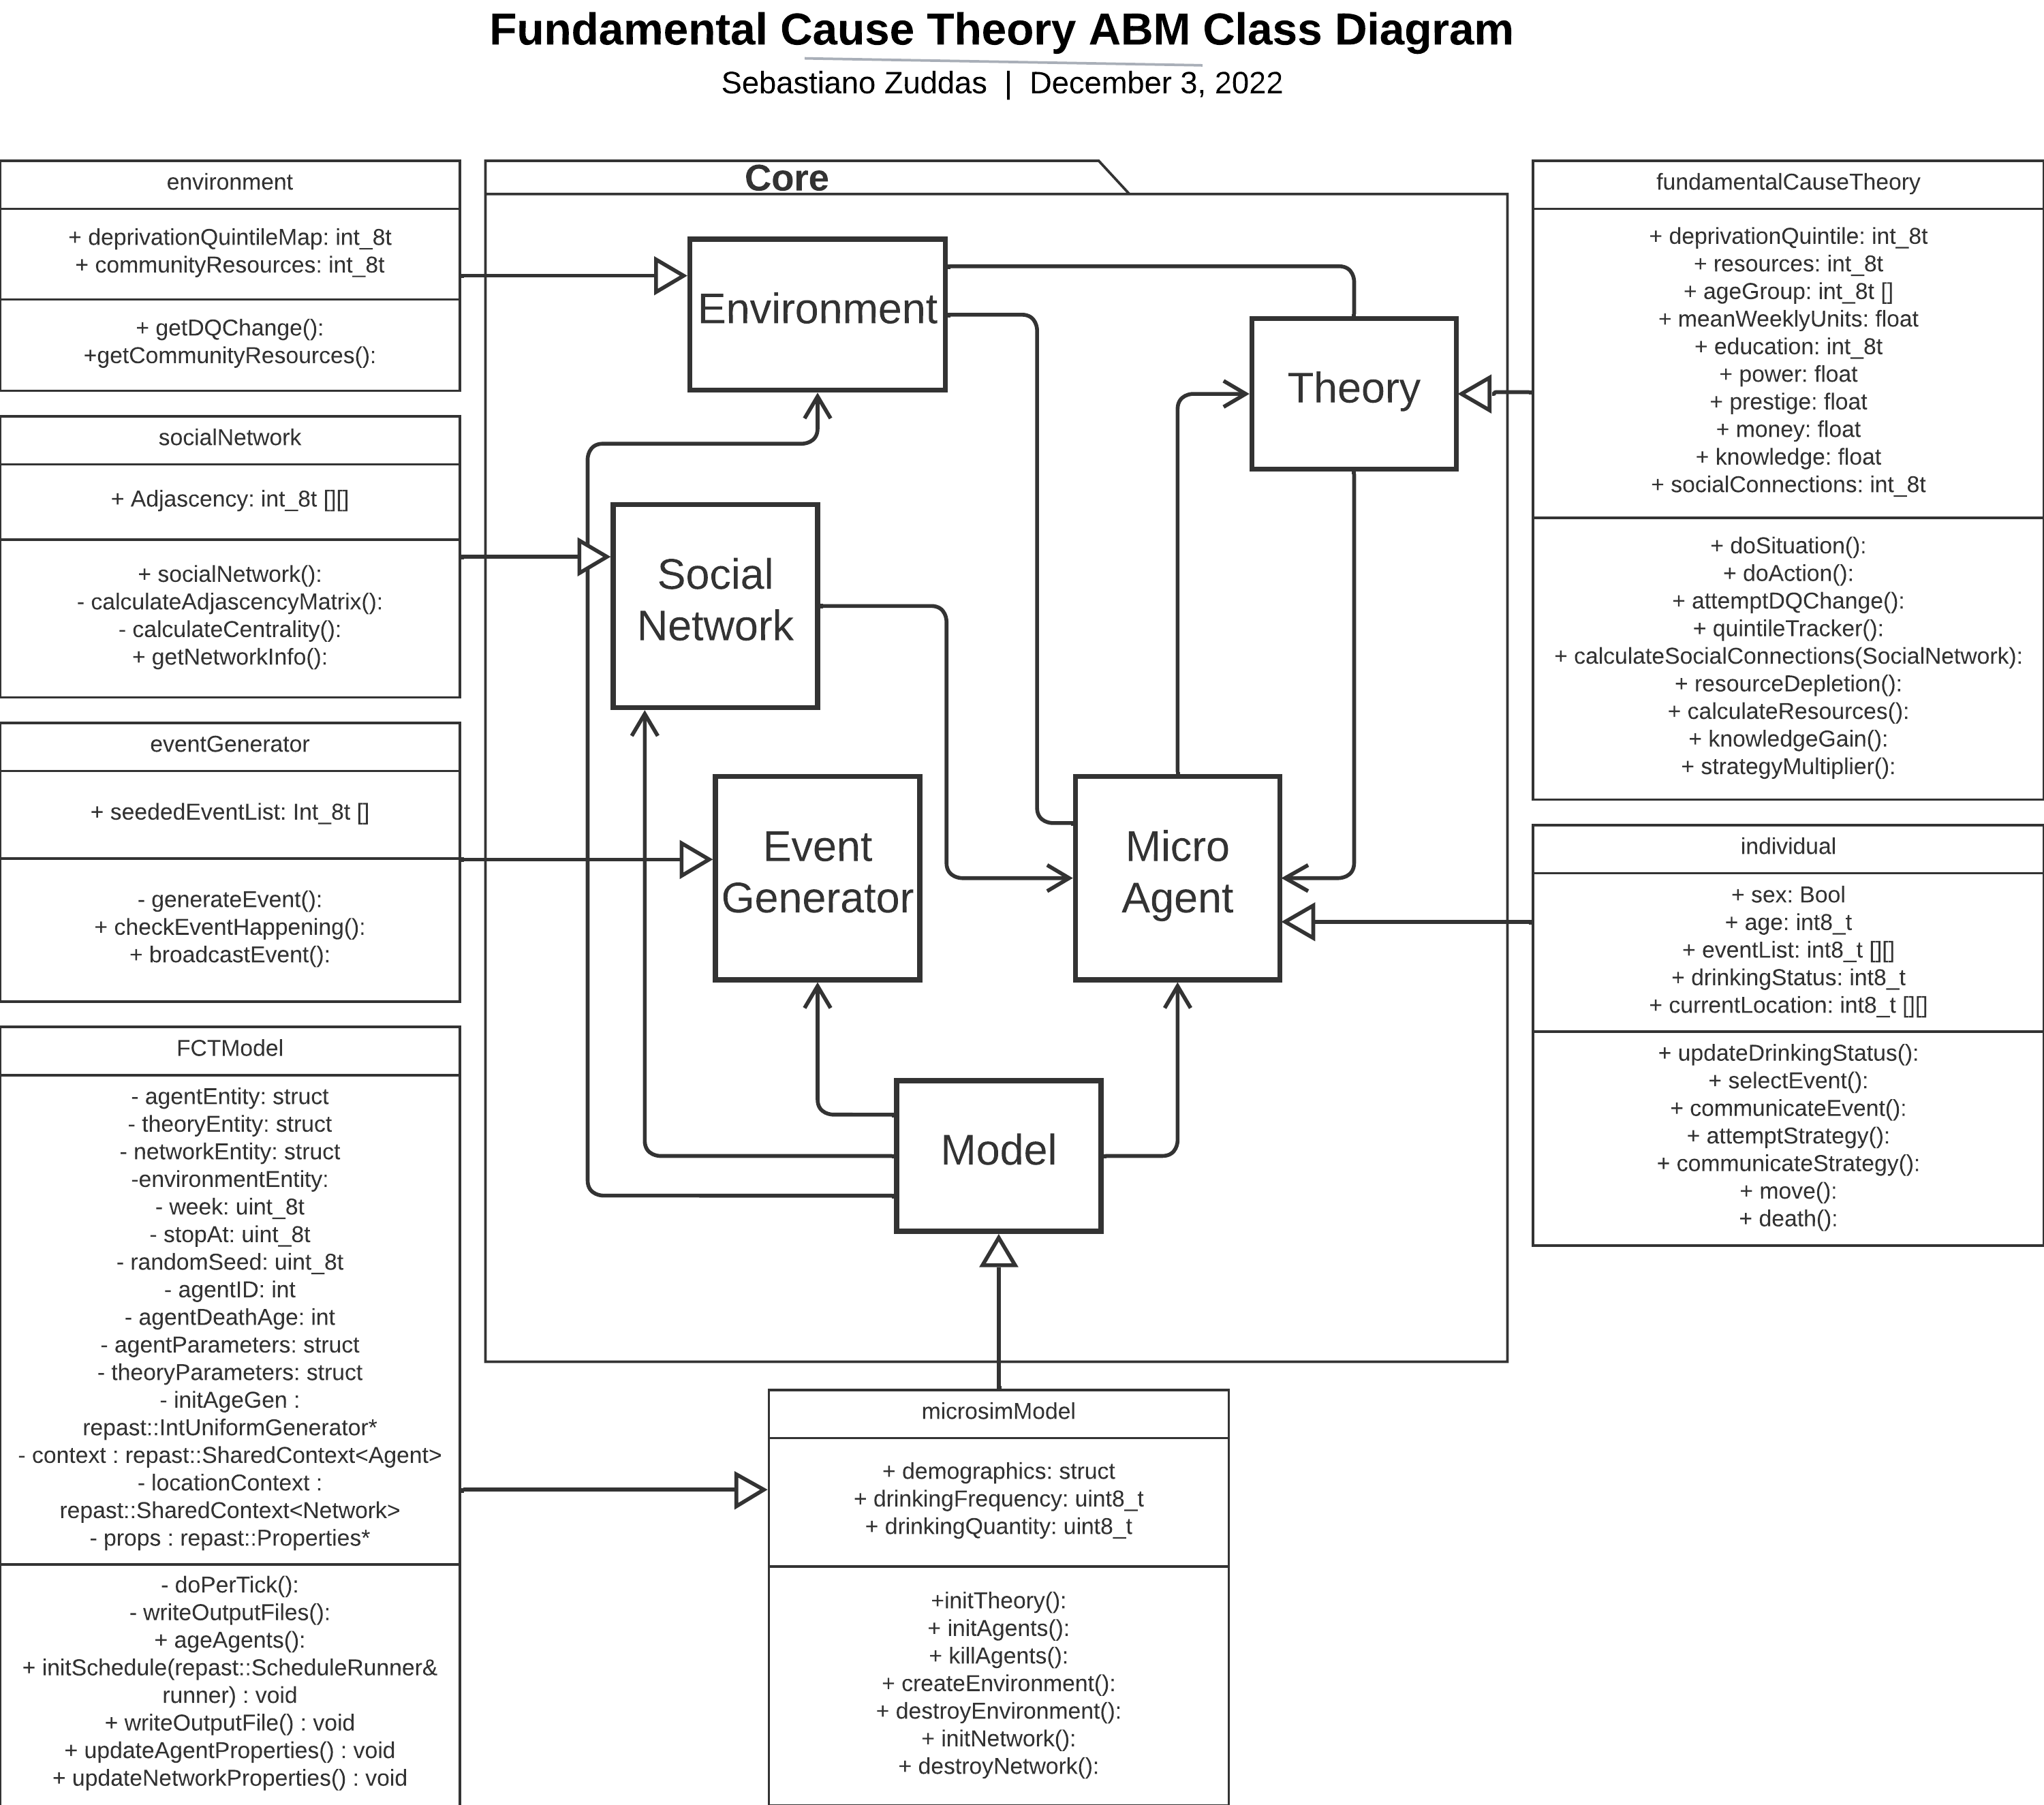
\includegraphics[width=\linewidth]{figures/Class Diagram FYP December.png}
\caption{A class diagram of the proposed ABM}
\label{fig:fctUML}
\end{figure}


% \subsection{Relevant Equations on Mechanisms of Action}
% \begin{figure}[h]
% \centering
% 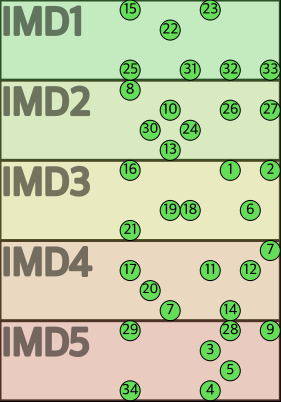
\includegraphics[scale=0.5]{USFD_Academic-_Report_LaTeX-Template/figures/ABM Diagram Single Year.png}
% \caption{An example graph}
% \label{fig:x cubed graph}
% \end{figure}


\subsection{Experiment Conceptualisation}

Table \ref{tab:experiments} shows a number of experiment concepts that has been reduced in the interest of keeping within the report requirements. The most important experiment that will be conducted is parameter space exploration through \ac{LHS}, a technique used to generate a set of parameters for this purpose. This is intended to demonstrate the general behaviour of the model and give insight into expected and unexpected behaviours. Other experiments, such as those related to \ac{FCT} and \ac{AHP} give credibility to the model. Finally, an interesting experiment would be to look at which \ac{FCT}-related parameters lead to the gratest harm, giving scope for further research and potential development for the model.  

\begin{table}[H]
\centering
\begin{tabular}{||p{0.3\textwidth}|p{0.3\textwidth}|p{0.3\textwidth}||}
 \hline
    Experiment & Method & Expected Impact \\[0.5ex] 
 \hline\hline
  Exploration of the parameter space. & Using \ac{LHS}. & Demonstrate general model behaviour. \\ 
  \hline
  Can \ac{FCT} be shown?  & Preventability shifts,  manipulated preventability. & Validation of \ac{FCT} working in the model. \\
  
  \hline
  Can \ac{AHP} be shown? & Changing the extremities of available community and individual resources & Further evidence that \ac{AHP} can be explained through \ac{FCT}. \\
  \hline
  
  Which \ac{FCT} parameters relate most to alcohol harm? & Test extremities of each \ac{FCT} parameter. & A certain combination of parameters will lead to the most harm for all individuals. \\ [1ex] 
 \hline
\end{tabular}
\caption{Table showing initial experiment concepts.}
\label{tab:experiments}
\end{table}

\section{Project Management \& Self Review}

\subsection{Gantt Chart \& Amendments}
The full pre-amendment Gantt chart can be found \href{https://www.notion.so/zuddas/9c097f57d9d844da8fc7f8733b38289f?v=61d021af0d9d40ebab7b2a6fbe6b3bd8}{here}. 
The full post-amendment Gantt chart can be found \href{https://www.notion.so/zuddas/ee42fe3d801947d08c59b69aa2e4f0cd?v=13936a7a4a4a4cff9e9fc01ff24508cb}{here}. 

Figure \ref{fig:S2Gantt} shows the amended Gantt chart for Semester 2. Amendments were made to extend the time allocated to the development, validation and appraisal of the \ac{ABM}. This was done to allow more than enough time to iron out related development problems related to making the model work in conjunction with surrounding software. There will be iterative development processes performed during the model development, firstly focusing on developing core aspects of the \ac{ABM} such as the agents themselves and their interactions with the environment and event generator. Gradually, development will expand to include the more complex features, such as the social network, as well as make the \ac{ABM} work with other software such as MATLAB to process inputs and outputs. 



\subsection{Self-Review}


Overall the project has seen good progress since the start of the semester. There has been excellent supervision and support on behalf of my supervisor. 

The research aspect of the project proved relatively challenging as there were many new concepts to learn in a field in which I had no expertise (public health). Nonetheless, I feel I have gained a relatively good understanding of the topics related to public health given the \ac{ABM} is the core focus of the project. There was less difficulty in apprehending concepts related to \ac{ABM} as it is a topic in which I was formally taught in the semester and had done some previous work on. 

There have been technical difficulties in using software and installing the various dependencies related to \ac{RHPC} both on my laptop and in the Linux remote server \cite{repasthpc}. This led to programming being slower than intended, and is a sign that work will have to be done over Christmas in order to compensate. The issues presented a challenge in understanding various computing concepts that were previously unknown to me, but they've extended my understanding of how computers work more generally. They are now mostly resolved and programming work can progress but there are still some issues that when overcome will lead to a more streamlined development process. 